\section{Question 5}
Consider the recurrent network shown below. Set the weights and biases in such a way that the network output remains 1 as long as the input sequence contains ones, and the network output changes to 0 when the input changes to 0. For example, the network output for the input sequence $x = 1111010000$ is $y = 1111000000$.
\begin{figure}[H]
    \centering
	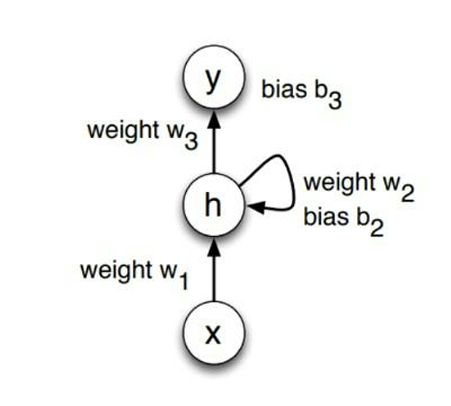
\includegraphics[width = 0.4\textwidth]{Q5.png}
	\caption{Recurrent network}
\end{figure}
\begin{qsolve}
	\begin{qsolve}[]
		The hidden state \( h_t \) acts as a memory cell. It needs to retain the value \( 1 \) if \( x_t = 1 \) or if the previous hidden state \( h_{t-1} \) was already \( 1 \). When \( x_t = 0 \), \( h_t \) should decay to \( 0 \). To achieve this, the hidden state can be defined as:
		\[
		h_t = \sigma(w_1 x_t + w_2 h_{t-1} + b_2),
		\]
		where \( \sigma(z) \) is the sigmoid activation function. Setting \( w_1 = 1 \), \( w_2 = 1 \), and \( b_2 = -0.5 \) ensures that \( h_t \) transitions smoothly. When \( x_t = 1 \), \( h_t \approx 1 \). When \( x_t = 0 \), \( h_t \) decays toward \( 0 \).
		
		The output \( y_t \) should mirror the value of the hidden state \( h_t \). The output is defined as:
		\[
		y_t = \sigma(w_3 h_t + b_3).
		\]
		To ensure \( y_t \approx 1 \) when \( h_t = 1 \) and \( y_t \approx 0 \) when \( h_t = 0 \), we can set \( w_3 = 10 \) and \( b_3 = -5 \). These values ensure a sharp transition between \( y_t = 1 \) and \( y_t = 0 \).
		
		using this configuration for the input sequence \( x = 1111010000 \), we get this output:
\[
y = 1111000000.
\]
	\end{qsolve}
\end{qsolve}